%% paper_rewritten_uk.tex -- Astronomy & Astrophysics manuscript
%%
%% This version has been rewritten in a more restrained A&A style, with
%% UK spelling conventions where appropriate. It assumes the official
%% A&A class file (aa.cls), aa.bst, and references.bib are available in
%% the Overleaf/project directory.

\documentclass{aa}

\usepackage{txfonts}
\usepackage{graphicx}
\usepackage{amsmath}
\usepackage{amssymb}
\usepackage{url}

\begin{document}

\title{Solar Orbiter/PHI polar magnetograms as standalone constraints on surface flux transport estimates of the Sun's axial dipole moment}

\author{M.~H.~Talafha\inst{1,2}}

\institute{
Research Institute of Sciences and Engineering, University of Sharjah, Sharjah, United Arab Emirates\\
\email{mtalafha901@gmail.com}
\and
HUN-REN Wigner Research Centre for Physics, Budapest, Hungary
}

\date{Received ---; accepted ---}

\abstract
{The Sun's axial dipole moment, $g_{10}$, is among the strongest observational precursors of the amplitude of the next activity cycle and provides a compact low-order measure of the large-scale field evolved by surface flux transport (SFT) models. Its value is controlled mainly by the polar field, precisely the region that near-ecliptic magnetographs such as SDO/HMI observe at unfavourable angles.}
{We investigate whether the out-of-ecliptic vantage of Solar Orbiter/PHI improves the observational constraint on the polar field and whether this information changes the SFT prediction obtained from Earth-view data alone.}
{We use a single open-source pipeline to construct PHI-only, HMI-only, and, where geometrically justified, merged Carrington maps. The HMI-only product is built in the native Earth-view geometry, while the merged product uses HMI reprojected to the PHI image plane. The axial dipole coefficient is evaluated under three polar-filling assumptions. We analyse a low-inclination validation window in CR\,2264 and the high-$B_0$ Solar Orbiter campaign from February to July 2025, covering CR\,2294--2299.}
{In CR\,2264 the independent products agree on the common support at the level of $\simeq0.05$\,G in $g_{10}$ and have a map-space correlation of $r\simeq0.89$, validating the pipeline. In the 2025 campaign, PHI's reliable ($\mu\ge0.4$) polar-cap coverage above $60^{\circ}$ exceeds HMI's by up to a factor of 16 (51\% versus 3\% in April 2025). This advantage appears and disappears with the difference between the Solar Orbiter and Earth heliographic latitudes. However, the largest polar advantage occurs at the largest Solar Orbiter--Earth longitude separations, where a per-pixel PHI--HMI merge is not meaningful. At the northern high-latitude apex, PHI gives a negative north-polar contribution to $g_{10}$, while the HMI grazing-angle estimate gives the opposite sign. Replacing the poorly observed HMI north cap with the PHI-derived cap in the SFT initial condition shifts the first predicted reversal by $-1.68$\,yr. By contrast, imposing the co-observed southern cap changes the timing by only $-0.004$\,yr.}
{The polar view affects the flux-transport prediction only where the Earth view lacks reliable information. Solar Orbiter/PHI is therefore most useful not as a co-registered merge partner for HMI at the decisive epochs, but as a standalone polar boundary constraint. The two vantages are complementary in time, not in space.}

\keywords{Sun: magnetic fields -- Sun: photosphere -- Sun: activity -- Sun: heliosphere -- methods: data analysis -- instrumentation: polarimeters}

\titlerunning{Solar Orbiter/PHI polar constraints on the axial dipole}
\authorrunning{M.~H.~Talafha}

\maketitle

%-------------------------------------------------------------------
\section{Introduction}
\label{sec:introduction}

The polar magnetic field near solar minimum is the best-known precursor of the amplitude of the following sunspot cycle \citep{Svalgaard2005,Petrovay2020}. Its low-order proxy, the axial dipole moment,
\begin{equation}
    g_{10} = \frac{3}{4\pi} \oint B_r \sin\lambda\,\mathrm{d}\Omega,
    \label{eq:g10-intro}
\end{equation}
where $\lambda$ is heliographic latitude, is a natural summary quantity for SFT studies \citep{Babcock1961,Leighton1969,Sheeley2005,WangSheeley1991,Wang2017}. An error in the polar field therefore enters solar-cycle predictions through the poloidal-field reservoir from which the next cycle's toroidal field is generated in Babcock--Leighton dynamo models \citep{CameronSchussler2015}.

The polar field is also the least favourably observed part of the solar surface. From near the ecliptic, the poles are seen at grazing angle ($\mu=\cos\theta\to0$, where $\theta$ is the heliocentric angle), so a line-of-sight measurement must be converted into a radial field through a large geometrical correction. In addition, for part of the year one pole is tilted away from Earth. Standard synoptic products, such as \texttt{hmi.synoptic\_mr\_polfil\_720s}, therefore fill the polar caps with a temporal or spatial model rather than with contemporaneous measurements alone \citep{Sun2018}. The polar contribution to $g_{10}$ is consequently a mixture of observation and assumption.

Solar Orbiter \citep{Muller2020} changes this observational geometry. Owing to repeated Venus gravity assists, its orbit is progressively inclined out of the ecliptic, and the Polarimetric and Helioseismic Imager (PHI; \citealp{Solanki2020}) can observe the photospheric magnetic field from heliolatitudes unavailable to Earth-view magnetographs. This provides a direct test of whether polar-view magnetic information modifies the inferred axial dipole and the SFT evolution that follows from it.

Previous comparisons of SO/PHI and SDO/HMI have mainly addressed cross-calibration, image-level consistency, or the construction of combined magnetic products. The emphasis here is different. We ask whether the out-of-ecliptic PHI view changes $g_{10}$ and its SFT propagation. This distinction is important because PHI and HMI are directly mergeable only while they share sufficient common support. The largest polar advantage occurs when the two spacecraft view largely different solar longitudes.

The paper is organised as follows. Section~\ref{sec:data} describes the SO/PHI-FDT and SDO/HMI observations and the two observing windows. Section~\ref{sec:methods} gives the construction of the Carrington maps, the dipole estimator, and the SFT experiments. Section~\ref{sec:results} presents the low-inclination validation and the 2025 high-latitude campaign. Sections~\ref{sec:discussion}--\ref{sec:conclusions} discuss the result, list the main limitations, and summarise the conclusions.

%-------------------------------------------------------------------
\section{Observations and data preparation}
\label{sec:data}

We use SO/PHI-FDT Level-2 line-of-sight magnetograms (\texttt{blos}) and SDO/HMI \texttt{hmi.M\_720s} line-of-sight magnetograms. For each PHI observation, the nearest HMI record in time is selected. A pair is retained only if the time offset is below 600\,s.

\subsection{SO/PHI-FDT line-of-sight magnetograms}
\label{sec:data-phi}

The Full Disc Telescope (FDT) channel of PHI aboard Solar Orbiter \citep{Solanki2020} provides Level-2 full-disk line-of-sight magnetic-field maps under the observable name \texttt{blos}. The \texttt{blos} quantity is derived from the inverted magnetic-field strength and inclination. The same release also provides continuum intensity, Stokes profiles, line-of-sight velocity, and vector magnetic-field products, but only \texttt{blos} is used in the present work.

The processed SO/PHI-FDT observations span two observing programmes. A subset of files lacks the \texttt{CUNIT1}/\texttt{CUNIT2} FITS keywords, and these units are patched automatically on load. Datasets acquired from 22~February 2025 onwards are generally on-board averages of three individual measurements, intended to improve the signal-to-noise ratio. Residual artefacts, including telemetry gaps, focus changes, imperfect flat-fielding, ghost and fringe signatures, and a dust-grain imprint most visible in continuum intensity, can remain. These caveats are relevant when small differences between PHI and HMI are interpreted in weak-field regions.

Each PHI magnetogram is treated as the reference member of a matched PHI--HMI pair. In the merged product, the nearest HMI magnetogram is reprojected onto the PHI image grid, so that the Solar Orbiter viewing geometry is preserved.

\subsection{SDO/HMI line-of-sight magnetograms}
\label{sec:data-hmi}

For the Earth-view reference we use line-of-sight magnetograms from HMI \citep{Scherrer2012} aboard SDO \citep{Pesnell2012}, specifically the \texttt{hmi.M\_720s} series. HMI observes the Fe\,\textsc{i} 6173\,\AA\ line, as does SO/PHI, and the cadence is sufficient for temporal matching to the PHI-FDT observations.

For merged and reprojected products, HMI is transformed to the PHI image plane using the WCS information in the FITS headers \citep{Thompson2006}. By contrast, the HMI-only product used in the vantage comparison is constructed in the native Earth-view geometry. This avoids giving the HMI-only baseline Solar Orbiter's viewing geometry, which would otherwise make the comparison circular.

\subsection{The two observing windows}
\label{sec:data-windows}

Two observing windows are considered (Table~\ref{tab:data}). The first is a low-inclination validation window in CR\,2264, covering 27~October--3~November 2022. It contains 24 matched PHI--HMI cases from two observing programmes. Eighteen of the cases have $|\Delta t|\le3$\,s and the maximum offset is 189\,s. During this window Solar Orbiter's disk-centre heliographic latitude, $B^{\rm SolO}_0$, ranged from $+7.09^{\circ}$ to $+7.44^{\circ}$, while Earth's $B^{\oplus}_0$ ranged from $+4.72^{\circ}$ to $+4.88^{\circ}$. Solar Orbiter trailed Earth by $40^{\circ}$--$45^{\circ}$ in Carrington longitude. This configuration provides only a small polar-viewing advantage, and is therefore used mainly to test the pipeline.

The second window is the high-$B_0$ Solar Orbiter campaign from 14~February to 16~July 2025, spanning CR\,2294--2299. The time matching is essentially simultaneous, with typical offsets of 2--3\,s. Over this interval $B^{\rm SolO}_0$ moved from near-ecliptic values ($-2.4^{\circ}$) to a deep southern view ($-16.7^{\circ}$), then to a northern plateau ($+16.8^{\circ}$), and finally back towards the ecliptic. At the same time, Earth's $B^{\oplus}_0$ rose from about $-7.2^{\circ}$, crossed zero, and reached about $+4.5^{\circ}$ by mid-July. The Solar Orbiter--Earth Carrington-longitude separation ranged from $0.3^{\circ}$ near conjunction to nearly $180^{\circ}$ near opposition. A single rotation contains up to 211 matched cases.

\begin{table}
\caption{Summary of the two observing windows.}
\label{tab:data}
\centering
\footnotesize
\begin{tabular}{lcc}
\hline\hline
Property & CR\,2264 & 2025 campaign \\
\hline
Rotations & CR\,2264 & CR\,2294--2299 \\
Start & 2022-10-27 & 2025-02-14 \\
End & 2022-11-03 & 2025-07-16 \\
Matched cases & 24 & 34--211 per rotation \\
Match tolerance & 600\,s & 600\,s \\
Typical $|\Delta t|$ & $\le3$\,s$^{a}$ & 2--3\,s \\
$B^{\rm SolO}_0$ range & $+7.1^{\circ}$ to $+7.4^{\circ}$ & $-16.7^{\circ}$ to $+16.8^{\circ}$ \\
$B^{\oplus}_0$ range & $+4.7^{\circ}$ to $+4.9^{\circ}$ & $-7.2^{\circ}$ to $+4.5^{\circ}$ \\
Separation & $40^{\circ}$--$45^{\circ}$ & $0.3^{\circ}$--$180^{\circ}$ \\
\hline
\end{tabular}
\tablefoot{$^{a}$ For 18 of 24 cases; the remaining cases reach 189\,s.}
\end{table}

\subsection{Time matching and viewing-geometry systematics}
\label{sec:data-systematics}

Two systematics related to viewing geometry are treated explicitly. First, the native HMI map path honours the full PC/CROTA orientation in the FITS header. Neglecting HMI's $\simeq180^{\circ}$ camera rotation mirrors the map between hemispheres and can change the sign of $g_{10}$; in the CR\,2264 subset, the project-mode value changes from $-2.11$ to $+2.20$\,G if this orientation is mishandled. Secondly, the line-of-sight field is converted to an approximate radial field using $B_r\simeq B_{\rm los}/\mu^{\alpha}$ with a limb cut, as described in Sect.~\ref{sec:methods-radial}.

Previous SO/PHI--HMI comparisons have established broad consistency between the two instruments for representative dates, both for SO/PHI-HRT \citep{Sinjan2023} and SO/PHI-FDT \citep{MorenoVacas2024}. Here, the check is performed case by case. A through-origin PHI-versus-HMI slope and a Pearson correlation coefficient are computed over common-support pixels satisfying a field-strength floor and $\mu\ge\mu_{\rm min}$. Over CR\,2264, the slope declines from about 0.75 to about 0.50 as the Solar Orbiter--Sun distance increases from 0.42 to 0.52\,AU, while the correlation remains near $r\simeq0.76$ (Fig.~\ref{fig:calibration}). A group of late-UT cases from 30--31~October falls below this trend, with slopes near 0.44--0.46 and correlations near 0.60. These cases are retained as diagnostics, but a correlation floor is used when calibration is applied.

In the 2025 campaign, the PHI--HMI slope is about 0.56 and the correlation about 0.8 while the two spacecraft co-observe. Once the Solar Orbiter--Earth separation exceeds about $55^{\circ}$, the common-support region moves to the limb and both quantities decrease rapidly. Calibration is therefore applied only when requested, only when the correlation exceeds the adopted floor, and only when the two spacecraft actually co-observe.

The sub-unity calibration slope is dominated by resolution-dependent flux cancellation rather than by a simple absolute scale offset. This is shown by smoothing the co-observed HMI map before the regression in the 112 CR\,2294 cases (Fig.~\ref{fig:resolution}). The mean slope rises from 0.56 to 0.63, 0.80, 0.88, 0.98, and 1.08 for Gaussian FWHM values of 0, 1, 2, 3, 5, and 8 PHI-grid pixels, respectively. The correlation peaks at FWHM 2--3 pixels, with $r\simeq0.93$. Thus, degrading HMI towards the effective PHI resolution both restores the scale and improves the correlation.

\begin{figure*}
\centering
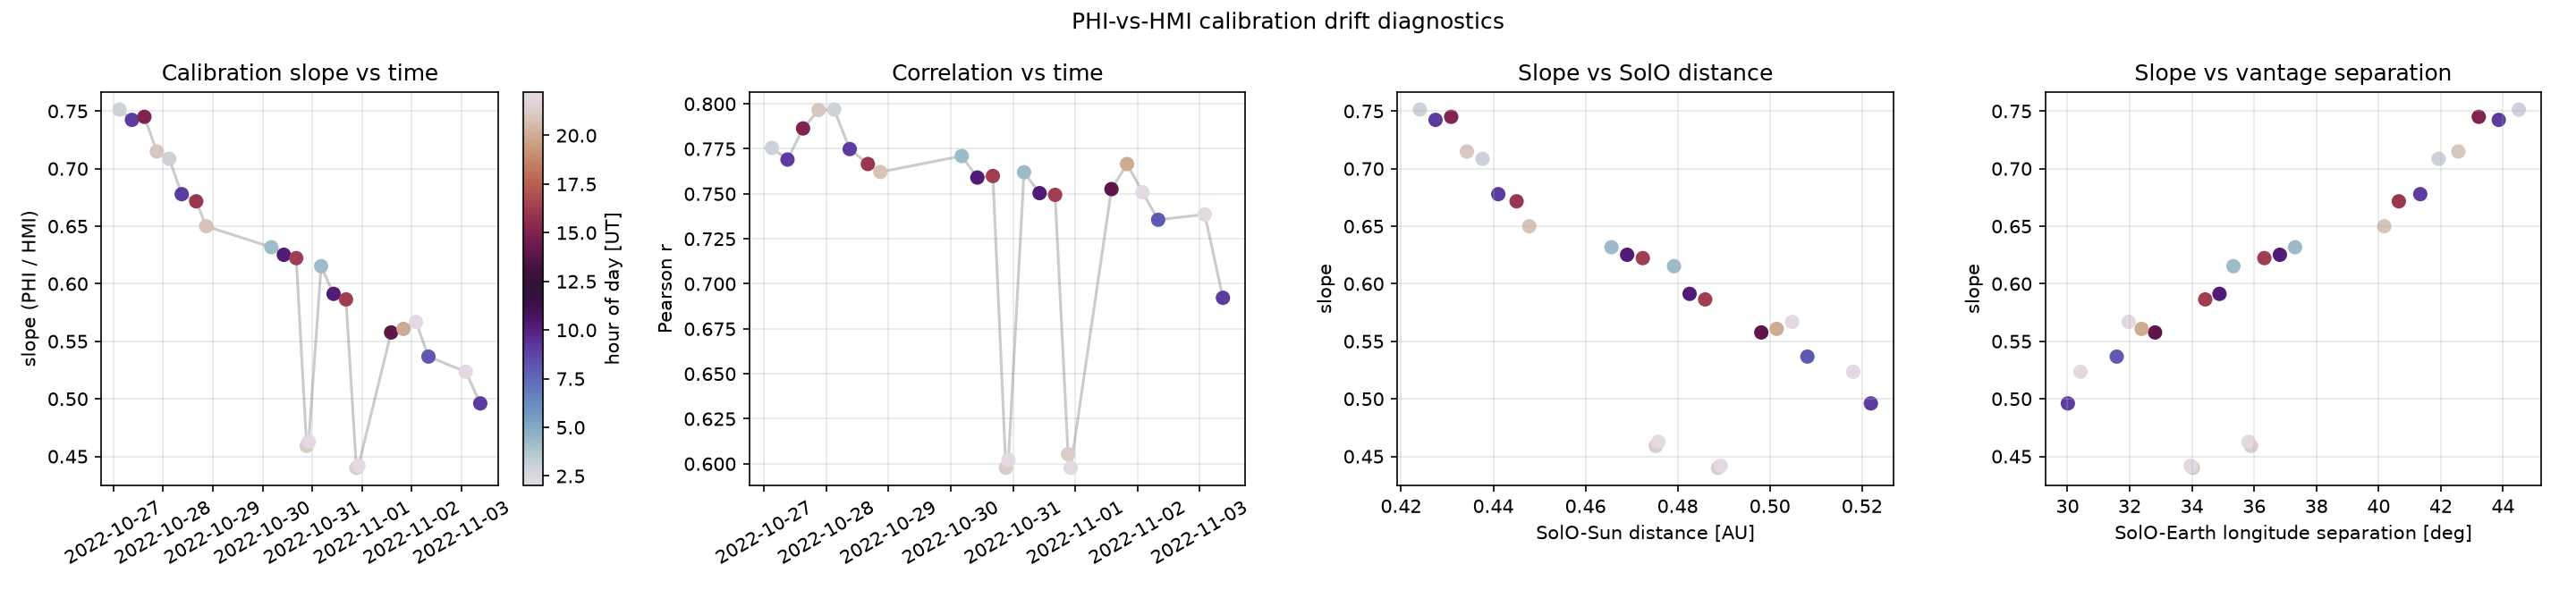
\includegraphics[width=0.98\textwidth]{figures/calibration_drift.png}
\caption{PHI-versus-HMI calibration diagnostics for CR\,2264, coloured by hour of day. From left to right: through-origin slope versus time, Pearson correlation coefficient versus time, slope versus Solar Orbiter--Sun distance, and slope versus Solar Orbiter--Earth longitude separation. Over this short window, time, distance, and separation are partly collinear; the slope correlates with these quantities, while the late-UT points form a lower-correlation observing-programme group. }
\label{fig:calibration}
\end{figure*}

\begin{figure}
\centering
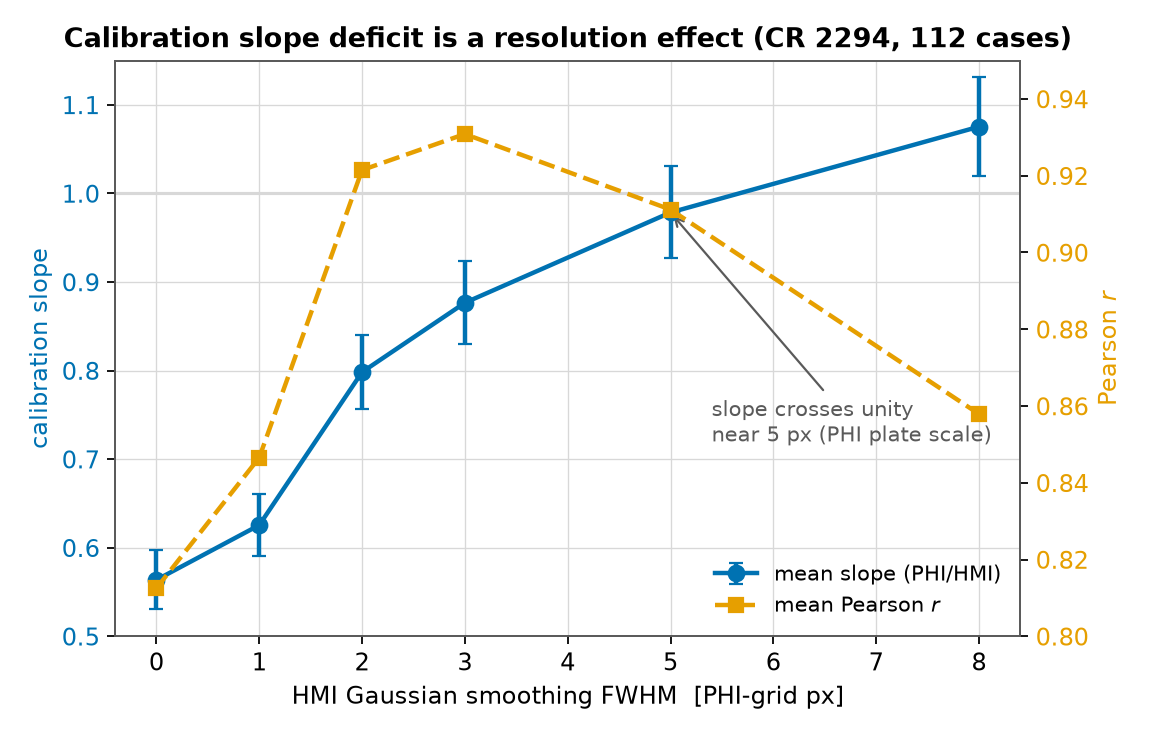
\includegraphics[width=\columnwidth]{figures/calibration_resolution.png}
\caption{Resolution test for the PHI-versus-HMI calibration slope in the 112 co-observing CR\,2294 cases. The HMI map is Gaussian-smoothed to a range of FWHM values, in PHI-grid pixels, before the through-origin regression. The slope rises to unity near 5 pixels, while the correlation peaks at 2--3 pixels. The result indicates that the slope deficit is largely produced by cancellation of fine mixed-polarity structure within the coarser PHI resolution element.}
\label{fig:resolution}
\end{figure}

%-------------------------------------------------------------------
\section{Methods: Carrington maps and the axial dipole estimator}
\label{sec:methods}

Combined SO/PHI and SDO/HMI synoptic magnetic-field products have been considered previously \citep{Loeschl2024a,Loeschl2024b}. The method used here is instead organised around individually matched full-disk observations. Each product is carried through the same steps: reprojection where needed, conversion to an approximate radial field, Carrington binning, evaluation of $g_{10}$, and SFT propagation.

\subsection{Reprojection and smooth radial blending}
\label{sec:methods-merge}

For each matched pair, the HMI magnetogram is reprojected onto the PHI grid using the WCS information in both FITS headers, with the SunPy and Astropy packages \citep{SunPy2020,Astropy2018}. The reprojection returns an HMI magnetic map sampled on PHI pixels and a footprint array marking where the transformation is defined. The quality of the transformation is checked both visually and through inner-disk pixel statistics, where limb-related interpolation errors are minimised.

A hard-boundary merge, in which one dataset is used inside a fixed disk radius and the other outside it, was tested first. It was found to be sensitive to the chosen switching radius, since a small change could include or exclude magnetically important regions and produce a non-monotonic change in the inferred dipole. We therefore adopted a smooth radial blend. Let $r$ be the normalised distance from disk centre in units of the apparent solar radius. The merged line-of-sight field is
\begin{equation}
    B_{\rm merge}(r) = w_{\rm PHI}(r) B_{\rm PHI}(r) + \left[1-w_{\rm PHI}(r)\right] B_{\rm HMI}(r),
    \label{eq:blend}
\end{equation}
where the PHI weight is defined by
\begin{equation}
    w_{\rm PHI}(r) =
    \begin{cases}
        1, & r \le R_{\rm inner}, \\[4pt]
        \frac{1}{2}\left[1+\cos(\pi x)\right], & R_{\rm inner}<r<R_{\rm outer}, \\[6pt]
        0, & r \ge R_{\rm outer},
    \end{cases}
    \label{eq:weight}
\end{equation}
with $x=(r-R_{\rm inner})/(R_{\rm outer}-R_{\rm inner})$. The baseline values are $R_{\rm inner}=0.70$ and $R_{\rm outer}=0.90$. PHI therefore dominates the central disk, HMI dominates the outer disk, and the transition is continuous. Pixels outside the HMI reprojection footprint are excluded from the HMI contribution. The merge is applied within an overall disk mask, \texttt{DISK\_FRACTION}=0.98, independently of the $\mu$ cut introduced below.

\subsection{Approximate conversion from line-of-sight to radial field}
\label{sec:methods-radial}

Because both PHI and HMI deliver line-of-sight fields, we use the approximate centre-to-limb correction
\begin{equation}
    B_r \simeq \frac{B_{\rm los}}{\mu^{\alpha}}, \qquad \mu=\cos\theta=\sqrt{1-r^2},
    \label{eq:br}
\end{equation}
retaining only pixels with $\mu\ge\mu_{\rm min}$. This approximation assumes that the large-scale photospheric field is predominantly radial. It is least reliable in strong active-region fields and near the limb, where division by powers of $\mu$ amplifies noise and projection errors.

The baseline values are $\mu_{\rm min}=0.40$ and $\alpha=0.8$. The exponent is not the dominant uncertainty in the tested range: over $\alpha=0.6$--1.0 the PHI dipole varies by about 3\% and the HMI dipole by about 9\%, both smaller than the case-to-case scatter. The choice of $\mu_{\rm min}$ is more important and can change the sign of single-vantage estimates. We therefore use $\alpha=0.8$ as a conservative alternative to the standard $1/\mu$ correction.

\subsection{Carrington binning and axial dipole}
\label{sec:methods-dipole}

Valid radial-field samples are assigned an approximate heliographic latitude $\lambda$ and Carrington longitude $\phi$ from the observer geometry in the map headers. They are then binned onto a regular $N_{\lambda}=180$, $N_{\phi}=360$ grid, corresponding to one degree per bin. Multiple cases within a Carrington rotation are combined with a central-meridian-distance weight, $\cos({\rm cmd})$, so that each observation contributes most strongly near its own central meridian.

From the binned map we compute
\begin{equation}
    g_{10} = \frac{3}{4\pi} \oint B_r \sin\lambda\,\mathrm{d}\Omega,
    \label{eq:g10}
\end{equation}
where $\mathrm{d}\Omega=\cos\lambda\,\mathrm{d}\lambda\,\mathrm{d}\phi$. The fill prescriptions are applied to the binned Carrington map before Eq.~(\ref{eq:g10}) is evaluated in discrete form. Three assumptions are considered for latitudes not sampled by a product: \emph{zero}, in which unobserved bins contribute nothing; \emph{project}, in which the observed field is least-squares projected onto the dipole profile; and \emph{polar\_extend}, in which unobserved polar caps are filled with the zonal mean of the last observed latitude band. We report these modes separately, since the fill mode is a major uncertainty on the absolute value of $g_{10}$. Product-to-product differences and coverage statistics are more robust.

Each product is stored together with a per-bin maximum-$\mu$ confidence grid. The HMI-only product is constructed in native Earth-view geometry, the PHI-only product in native Solar Orbiter geometry, and the merged product only when common support exists.

\subsection{Separation guard for the merged product}
\label{sec:methods-guard}

The merged product of Eq.~(\ref{eq:blend}) is meaningful only when the two spacecraft observe a common disk region. We therefore impose a maximum Solar Orbiter--Earth Carrington-longitude separation of $60^{\circ}$. This value follows from the observed collapse of the common-support calibration statistics beyond about $55^{\circ}$ in the 2025 campaign. A case beyond the threshold still contributes to the PHI-only and HMI-only native-geometry products, but it is excluded from the merged map and is not cross-calibrated.

This guard is central to the interpretation. The PHI polar advantage is largest at the epochs when the spacecraft separation is largest. At those epochs, a merged product would combine two largely disjoint hemispheres and would not represent a co-observed field. The appropriate result is therefore an empty merged map, not a forced blend.

Because the 2025 interval spans several Carrington rotations, all campaign products are analysed rotation by rotation. A single map over the full multi-month interval would mix different phases of the axial dipole evolution.

\subsection{One-dimensional surface flux transport model}
\label{sec:methods-sft}

To propagate the magnetic products forward, we use a one-dimensional axisymmetric SFT model of the Babcock--Leighton type \citep{Babcock1961,Leighton1969,Sheeley2005}. In colatitude $\theta$, the zonally averaged radial field obeys
\begin{equation}
\frac{\partial B}{\partial t} =
-\frac{1}{R_{\odot}\sin\theta}
\frac{\partial}{\partial\theta}\left[u(\theta)B\sin\theta\right]
+\frac{\eta}{R_{\odot}^{2}\sin\theta}
\frac{\partial}{\partial\theta}
\left(\sin\theta\frac{\partial B}{\partial\theta}\right)
-\frac{B}{\tau}+S(\theta,t).
\label{eq:sft}
\end{equation}
The numerical implementation uses the $W=R_{\odot}\sin\theta\,B$ formulation \citep{WangSheeley1991}. Differential rotation does not appear after longitudinal averaging. The transport parameters are a van-Ballegooijen-type meridional flow with amplitude $u_0=11$\,m\,s$^{-1}$, diffusivity $\eta=250$\,km$^2$\,s$^{-1}$ \citep{vanBallegooijen1998,Wang2017}, and decay time $\tau=10$\,yr in the cycle-source runs. The finite-difference code reproduces the analytic $\ell=1$ diffusive decay rate, $2\eta/R_{\odot}^{2}$, to better than 2\%.

\begin{table}
\caption{Parameters used in the one-dimensional SFT experiments.}
\label{tab:sft-params}
\centering
\footnotesize
\begin{tabular}{lc}
\hline\hline
Quantity & Value \\
\hline
Meridional-flow amplitude & $u_0=11$\,m\,s$^{-1}$ \\
Turbulent diffusivity & $\eta=250$\,km$^2$\,s$^{-1}$ \\
Decay time in cycle runs & $\tau=10$\,yr \\
Integration length & 22\,yr \\
Initial condition & zonal mean of map product \\
Flux balancing & global net-flux removal before injection \\
Reversal criterion & first zero crossing of $g_{10}(t)$ \\
\hline
\end{tabular}
\end{table}

Each magnetic product is injected as a zonal profile $B(\lambda)$ after global net-flux removal. Latitudes not observed by a single-vantage product are assigned $B=0$, so the missing-polar-field limitation is carried into the SFT initial condition. Two injection modes are used. \emph{Whole-map injection} uses the zonal average of a complete PHI-only, HMI-only, or merged map; it is appropriate only when the merged map is geometrically meaningful. \emph{Polar-constraint splicing} retains the HMI profile outside the selected polar cap, but replaces the cap with the PHI-derived zonal field through a smooth latitudinal ramp. This second mode is used for the high-separation 2025 rotations, where PHI constrains a pole that HMI observes only poorly.

%-------------------------------------------------------------------
\section{Results}
\label{sec:results}

\subsection{Low-inclination validation: CR\,2264}
\label{sec:results-demo}

CR\,2264 is used as a method demonstration rather than as a decisive polar-view test. Solar Orbiter led Earth in $B_0$ by only about $2.5^{\circ}$, and the two instruments retained substantial common support. The PHI and HMI products agree on $g_{10}$ to about 0.05\,G on this support (zero-fill mode: $-0.18$\,G for PHI and $-0.23$\,G for HMI), and the maps correlate at $r=0.89$ (Fig.~\ref{fig:maps2264}). This validates the orientation handling, calibration diagnostics, Carrington binning, and SFT coupling in a controlled geometry.

Against the standard HMI polar-filled synoptic chart for the same rotation, $g_{10,{\rm ref}}=+0.65$\,G, the PHI project-mode estimate differs by $+0.04$\,G (6\%). The best HMI-only fill mode in the same pipeline differs by 0.22\,G, about five times more. This ordering follows the available polar-cap fill, but the low-$B_0$ geometry means that the result is interpreted mainly as a pipeline check.

\begin{figure*}
\centering
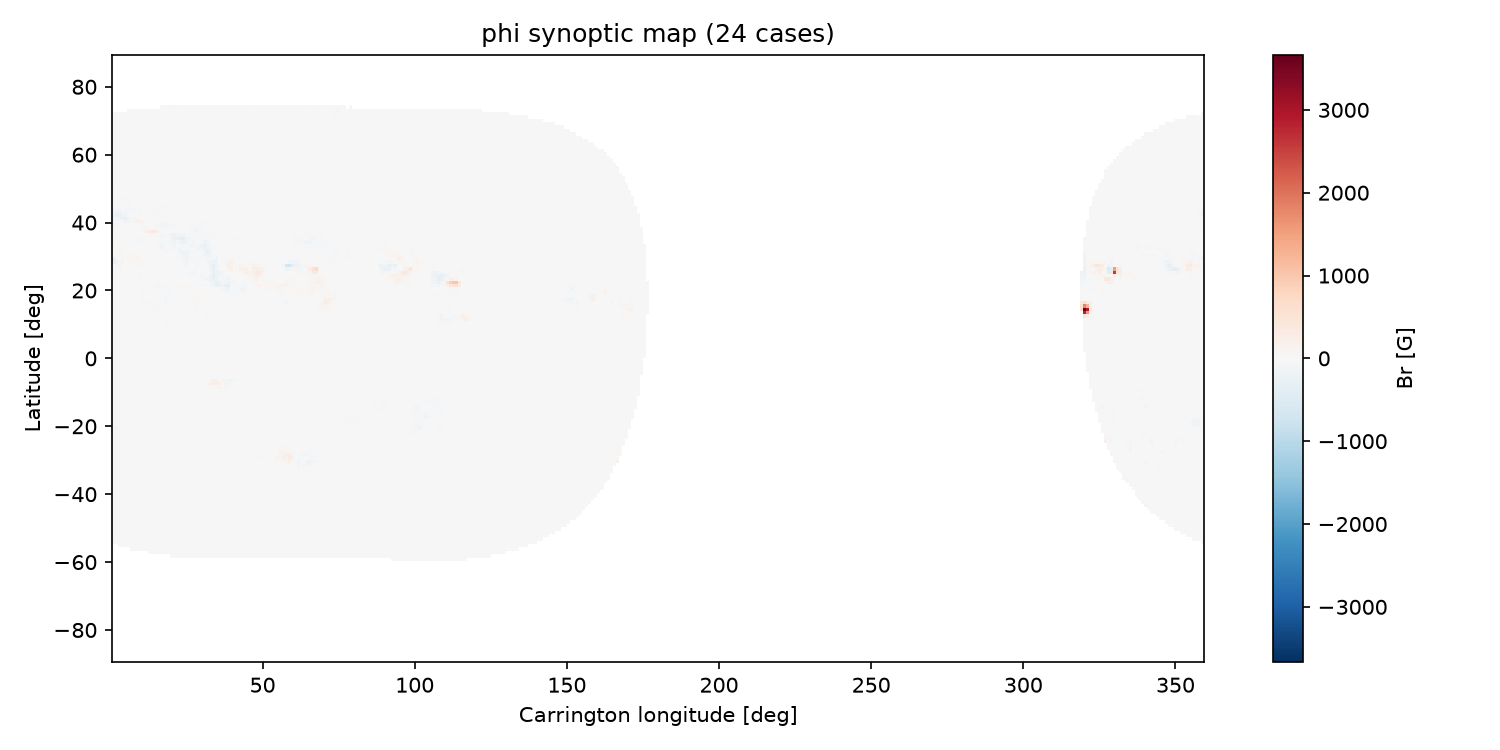
\includegraphics[width=0.32\textwidth]{figures/maps_cr2264_phi.png}\hfill
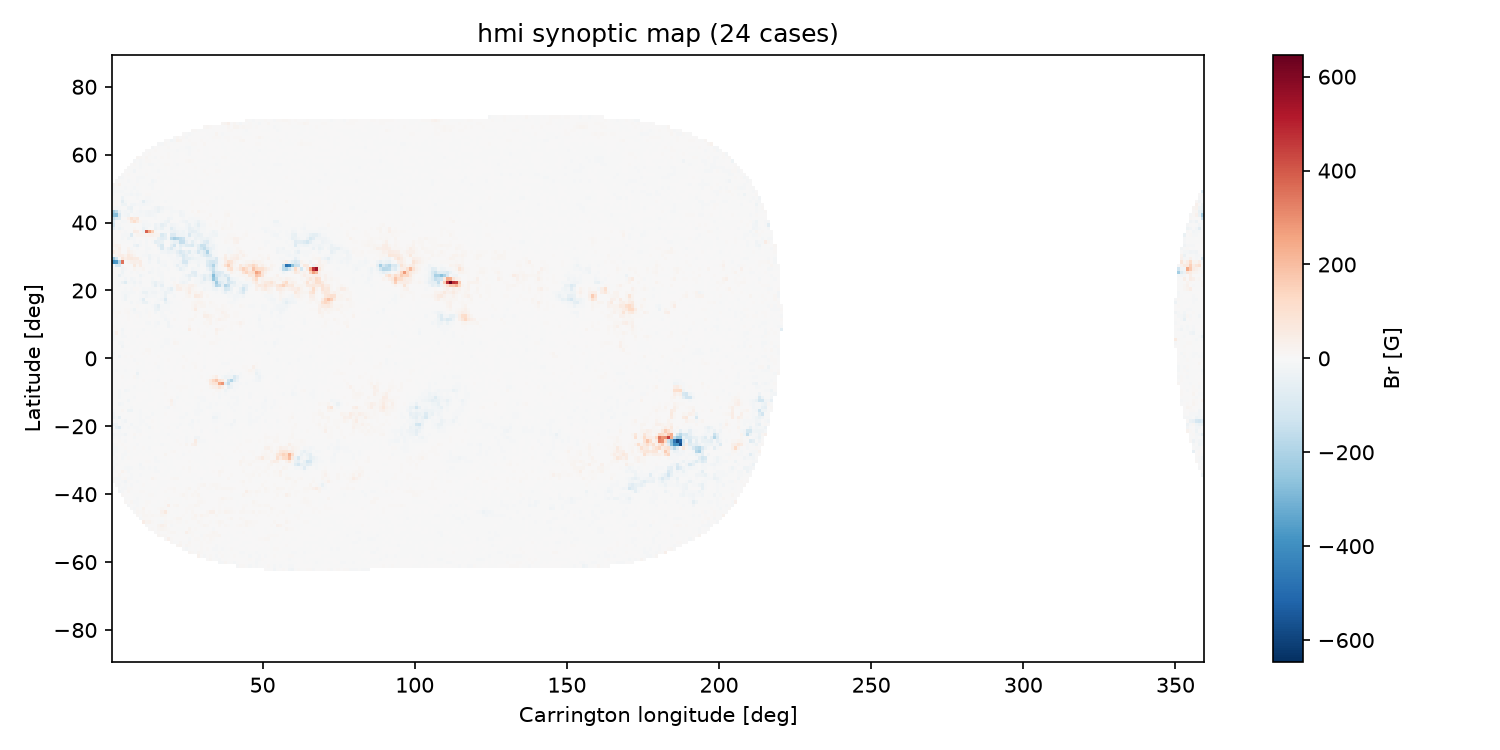
\includegraphics[width=0.32\textwidth]{figures/maps_cr2264_hmi.png}\hfill
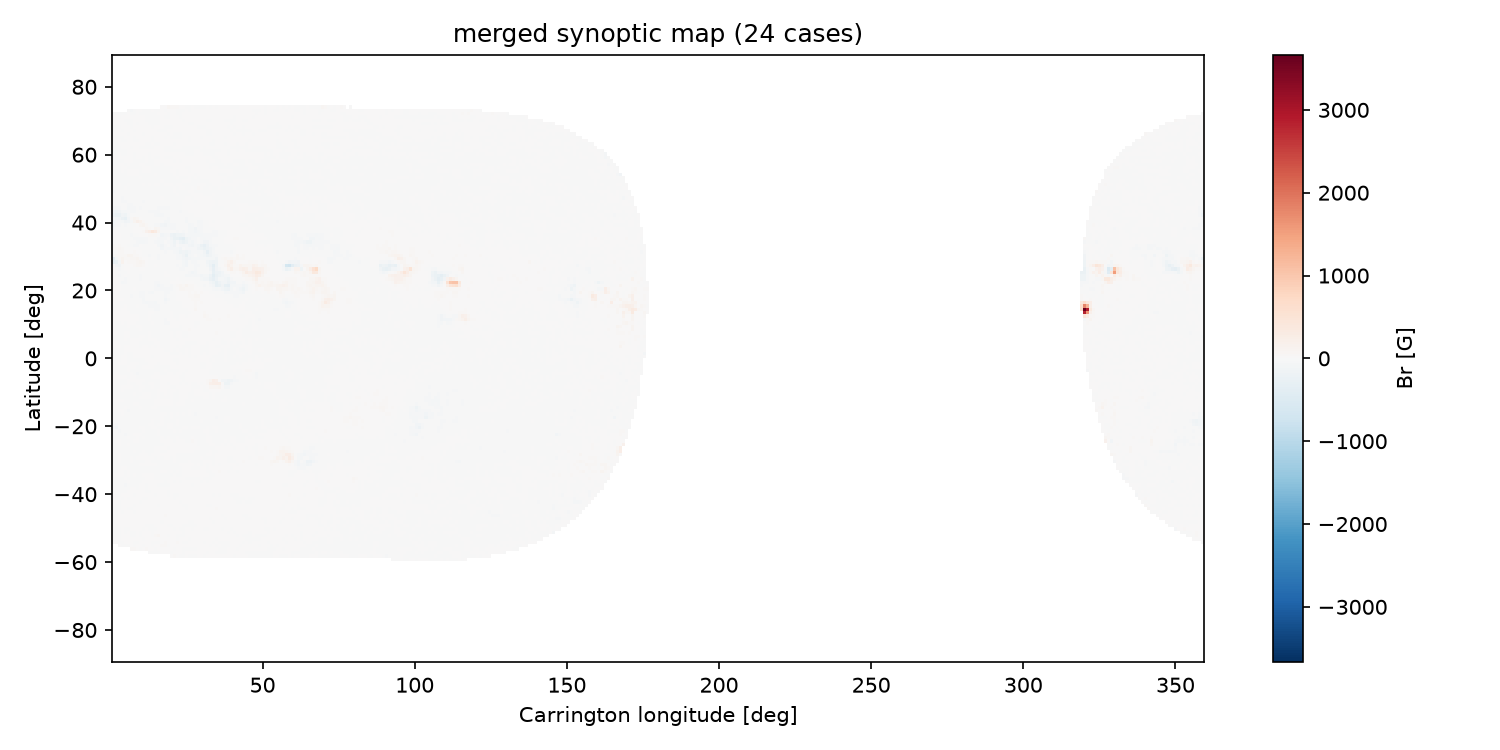
\includegraphics[width=0.32\textwidth]{figures/maps_cr2264_merged.png}
\caption{Radial-field ($B_r$) Carrington maps for the low-$B_0$ CR\,2264 demonstration: PHI-only (left), HMI-only in native Earth-view geometry (centre), and the smooth merge (right). At this modest Solar Orbiter--Earth separation the two vantages overlap, the common-support map correlation is $r=0.89$, and the merge is well posed.}
\label{fig:maps2264}
\end{figure*}

With a cycle source, the SFT runs show how differences in the initial map propagate into the early evolution. The first polar reversal occurs at 3.72\,yr for the PHI-informed initial condition and at 2.46\,yr for the HMI-only condition, a delay of 1.26\,yr relative to HMI\@. The 22-yr final dipoles converge to $+3.41$, $+3.17$, and $+3.40$\,G for the PHI, HMI, and merged initial conditions, respectively. Thus, the CR\,2264 run demonstrates the map-to-SFT propagation mechanism; the decisive polar-view test is provided by the 2025 campaign.

\subsection{The 2025 high-$B_0$ campaign: polar coverage}
\label{sec:results-coverage}

During 14~February--16~July 2025, Solar Orbiter's $B_0$ changed from $-2.4^{\circ}$ to $-16.7^{\circ}$, then to $+16.8^{\circ}$, and finally back towards the ecliptic. Earth moved from $B_0\simeq-7.2^{\circ}$, crossed zero in the later rotations, and reached $+4.5^{\circ}$ by mid-July. The polar-cap fill fractions above $60^{\circ}$ follow these viewing geometries directly (Table~\ref{tab:campaign}; Fig.~\ref{fig:campaign}).

\begin{table*}
\caption{Polar-cap coverage ($\ge60^{\circ}$, \%) and merge validity during the 2025 campaign. The values are computed per Carrington rotation with the conservative limb cut $\mu_{\rm min}=0.4$.}
\label{tab:campaign}
\centering
\scriptsize
\begin{tabular}{llcccccc}
\hline\hline
Rotation & Dates & Cases/merge & $B_0^{\rm SolO}$ & $B_0^{\oplus}$ & Separation & N-cap PHI/HMI & S-cap PHI/HMI \\
\hline
CR\,2294 & Feb 14--Mar 1  & 112/112 & $-2.4^{\circ}\rightarrow -7.7^{\circ}$  & $-6.8^{\circ}\rightarrow -7.2^{\circ}$  & $15.4^{\circ}$--$20.9^{\circ}$   & 5 / 0   & 30 / 37 \\
CR\,2295 & Mar 2--Mar 28  & 57/56   & $-7.7^{\circ}\rightarrow -16.7^{\circ}$ & $-6.7^{\circ}\rightarrow -7.3^{\circ}$  & $0.3^{\circ}$--$60.3^{\circ}$  & 0 / 0   & \textbf{64 / 46} \\
CR\,2296 & Mar 31--Apr 24 & 34/0    & $-8.2^{\circ}\rightarrow +16.6^{\circ}$ & $-6.6^{\circ}\rightarrow -4.8^{\circ}$  & $80.1^{\circ}$--$165.4^{\circ}$  & \textbf{51 / 3}  & 12 / 41 \\
CR\,2297 & Apr 26--May 22 & 211/0   & $+14.2^{\circ}\rightarrow +16.8^{\circ}$ & $-4.7^{\circ}\rightarrow -1.8^{\circ}$ & $167.6^{\circ}$--$180.0^{\circ}$ & \textbf{77 / 13} & 0 / 34 \\
CR\,2298 & May 23--Jun 19 & 152/0   & $+14.2^{\circ}\rightarrow +9.1^{\circ}$  & $-1.7^{\circ}\rightarrow +1.6^{\circ}$ & $178.9^{\circ}$--$180.0^{\circ}$ & 64 / 23 & 0 / 24 \\
CR\,2299 & Jun 20--Jul 16 & 198/0   & $+9.1^{\circ}\rightarrow +3.1^{\circ}$   & $+1.6^{\circ}\rightarrow +4.5^{\circ}$ & $175.2^{\circ}$--$179.0^{\circ}$  & 45 / 34 & 4 / 13 \\
\hline
\end{tabular}
\tablefoot{The ``Cases/merge'' column gives the number of matched PHI--HMI cases and the number retained in the merged product after applying the $60^{\circ}$ separation guard. The cap columns give PHI/HMI fill fractions in percent.}
\end{table*}

Near the ecliptic (CR\,2294), PHI has little polar advantage. As Solar Orbiter moves to negative heliolatitudes (CR\,2295), PHI's south-cap coverage exceeds HMI's (64\% versus 46\%). As the spacecraft crosses to a northern view, PHI becomes the better north-cap constraint: in CR\,2296 the north-cap fill is 51\% for PHI and 3\% for HMI, and in CR\,2297 it is 77\% and 13\%, respectively. As Solar Orbiter descends from the northern apex, PHI's north-cap fill decreases to 64\% in CR\,2298 and 45\% in CR\,2299, while HMI's increases to 23\% and 34\% as Earth's $B_0$ rises. Thus, the advantage is governed by the difference between the two heliolatitudes and switches on and off with that difference.

The merged product remains empty from CR\,2296 to CR\,2299. This is expected, because the Solar Orbiter--Earth separation remains large even while the polar-coverage advantage evolves. The polar-coverage effect is controlled by $B_0$, whereas merge validity is controlled by longitude separation. Since the coverage fractions are simple counts of observed bins, they do not depend on calibration or on the polar-fill assumption.

\begin{figure}
\centering
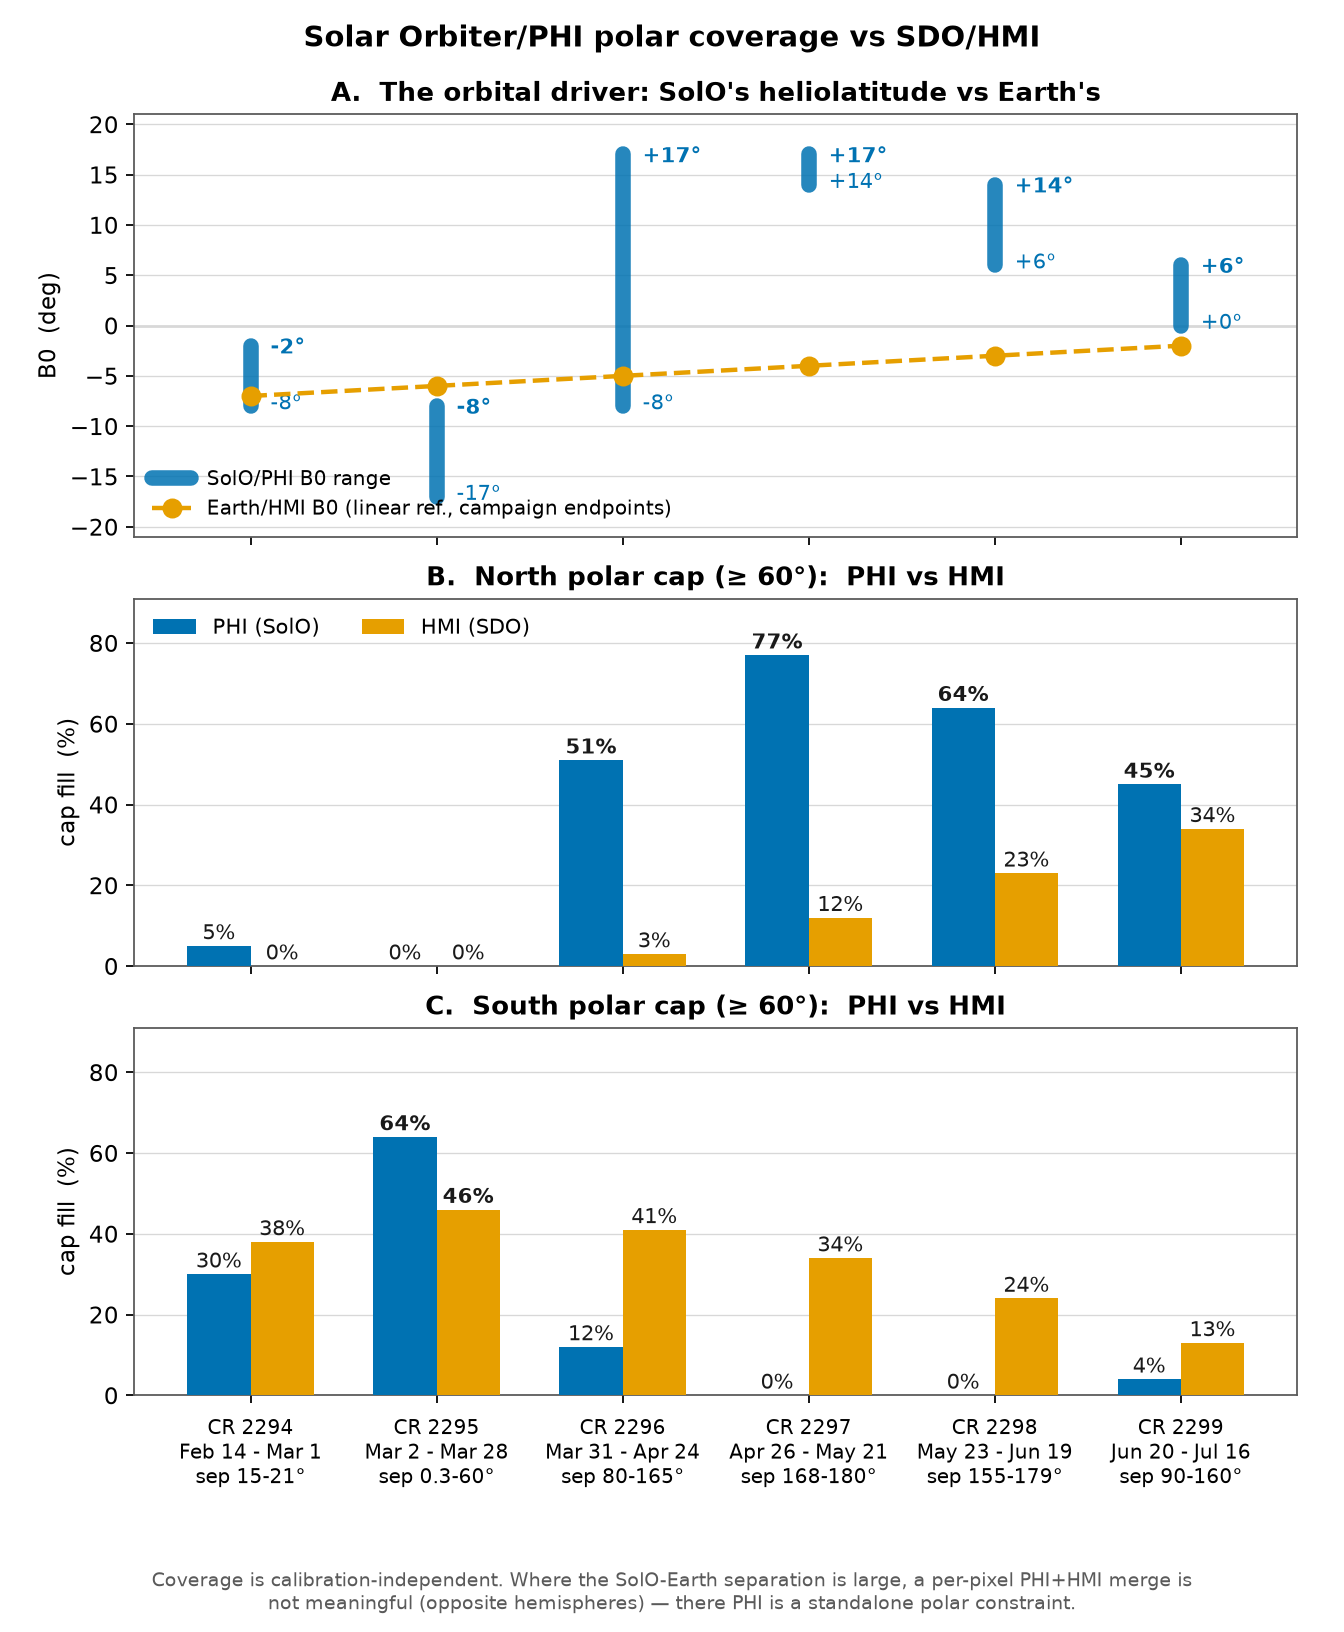
\includegraphics[width=\columnwidth]{figures/campaign_polar_advantage.png}
\caption{Solar Orbiter $B_0$ excursion and PHI-versus-HMI north/south polar-cap fill per rotation during the 2025 campaign, with the Solar Orbiter--Earth separation range indicated (Table~\ref{tab:campaign}). The values are derived from the per-rotation calibration tables.}
\label{fig:campaign}
\end{figure}

Table~\ref{tab:campaign} uses the conservative cut $\mu_{\rm min}=0.4$, corresponding to pixels within about $66^{\circ}$ of disk centre. The sign of the polar-coverage advantage is robust, but its magnitude depends on how much limb extrapolation is permitted. For example, at $\mu_{\rm min}=0.25$ the CR\,2296 north-cap fill rises from 3\% to 33\% for HMI and from 51\% to 86\% for PHI, so the ratio decreases from about $16\times$ to about $2.6\times$. PHI still leads. The order-of-magnitude advantage therefore refers to reliable high-$\mu$ polar coverage, where HMI contributes almost no usable pixels while PHI observes the cap closer to disk centre.

\subsection{Vantage effect on the dipole}
\label{sec:results-sign}

The effect of the different vantage points is also seen in the polar contribution to $g_{10}$. On the common polar support of CR\,2295, the project-mode south-polar contribution has opposite signs for the two instruments: $+0.21$\,G for PHI and $-0.10$\,G for HMI on the same bins. A positive calibration factor cannot change the sign, so this difference is a geometrical effect. In that interval, HMI views the south cap close to the limb, while PHI observes it closer to disk centre.

The clearest sign test occurs in CR\,2297. PHI maps 77\% of the north cap, whereas HMI maps only 13\% at grazing angle. The PHI north-polar contribution is negative, $g_{10,{\rm north}}=-0.254$\,G, while the HMI contribution is positive, $+0.191$\,G (Table~\ref{tab:northsign}). The standard HMI polar-filled synoptic chart for the same rotation has a negative total dipole, $g_{10}=-0.388$\,G. Thus, the polar-view measurement recovers the expected polarity of the reversing cycle-25 north polar field, while the near-blind Earth-view extrapolation gives the opposite cap contribution.

\begin{table}
\caption{North-polar contribution to the project-mode dipole in CR\,2297.}
\label{tab:northsign}
\centering
\footnotesize
\begin{tabular}{lcc}
\hline\hline
Product & N-cap fill & $g_{10,{\rm north}}$ \\
\hline
PHI & 76.6\% & $-0.254$\,G \\
HMI & 12.6\% & $+0.191$\,G \\
HMI polar-filled reference & -- & negative total $g_{10}$ ($-0.388$\,G) \\
\hline
\end{tabular}
\tablefoot{The PHI and HMI rows give the north-hemisphere contribution from the project-fill decomposition of the native-geometry Carrington products. The reference row gives the total dipole of the HMI polar-filled synoptic chart for the same rotation and is used only as a sign check.}
\end{table}

\begin{figure*}
\centering
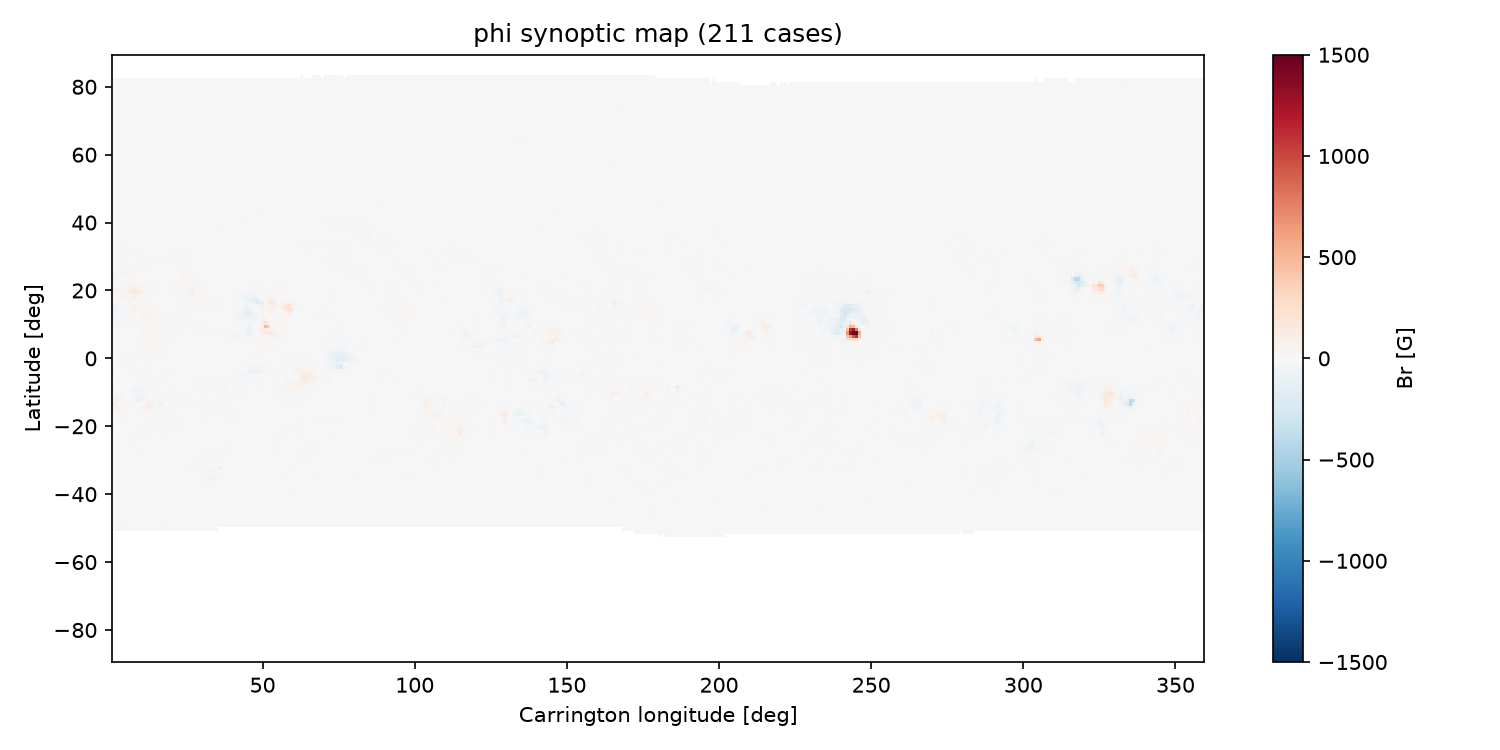
\includegraphics[width=0.32\textwidth]{figures/maps_cr2297_phi.png}\hfill
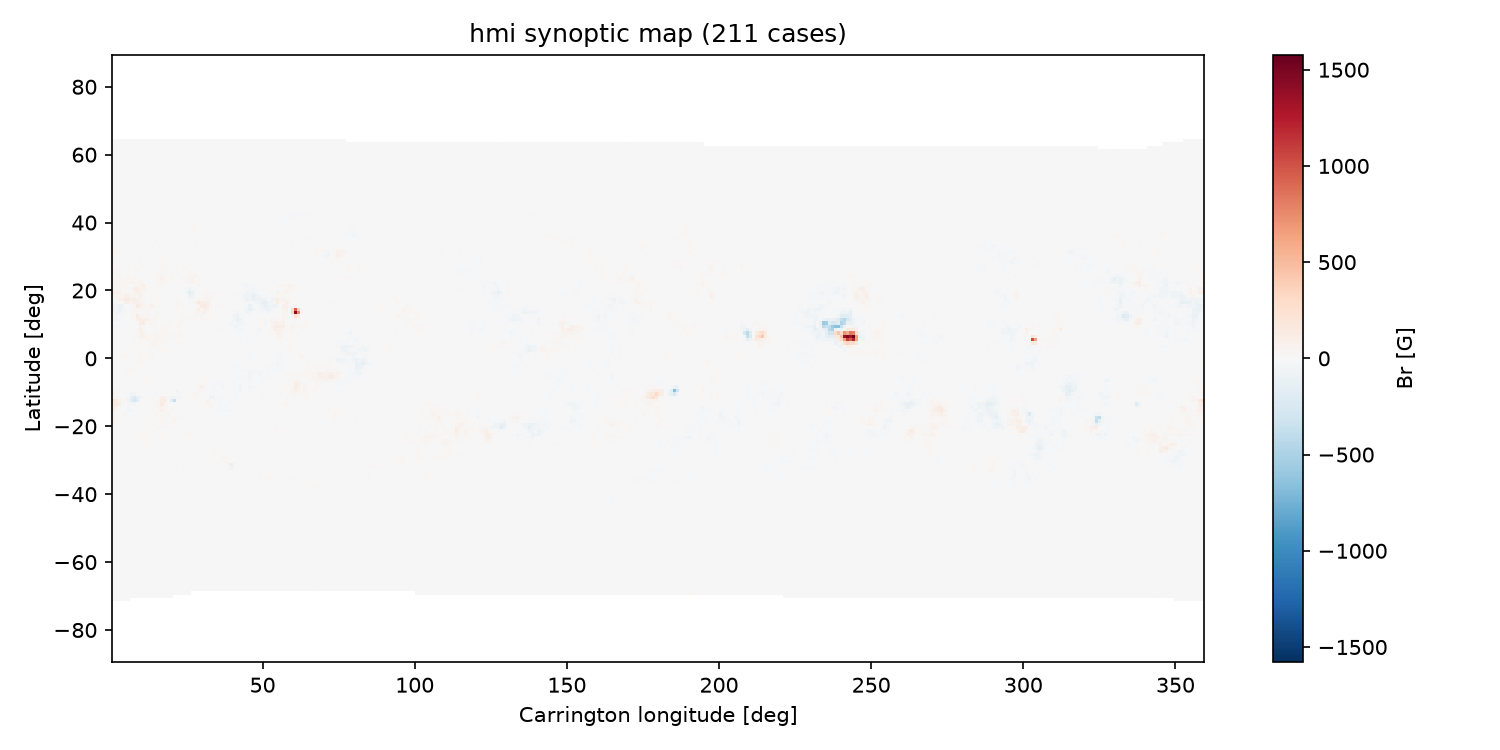
\includegraphics[width=0.32\textwidth]{figures/maps_cr2297_hmi.png}\hfill
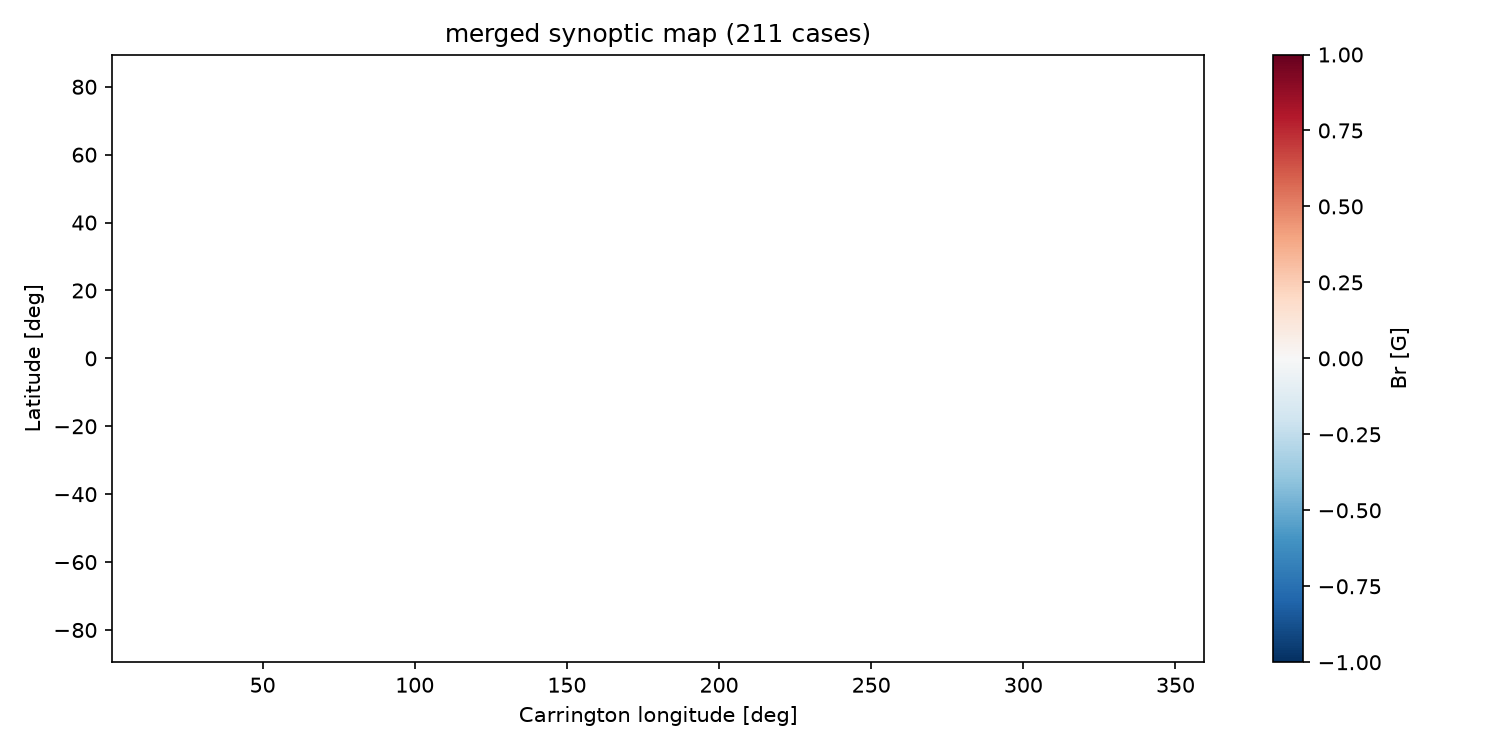
\includegraphics[width=0.32\textwidth]{figures/maps_cr2297_merged.png}
\caption{Radial-field ($B_r$) Carrington maps for the high-$B_0$ CR\,2297 rotation: PHI-only (left), HMI-only in native Earth-view geometry (centre), and the merged product (right). PHI populates 77\% of the north polar cap, while HMI samples only 13\% at grazing angle. The merged product is empty because the Solar Orbiter--Earth separation is $167.6^{\circ}$--$180.0^{\circ}$, leaving no co-observed disk within the separation guard. The empty panel therefore denotes an invalid merged product, not zero magnetic field.}
\label{fig:mapshighb0}
\end{figure*}

\subsection{SFT impact of the PHI polar constraint}
\label{sec:results-sft}

Since a per-pixel merge is invalid in the high-$B_0$ rotations, PHI is injected as a polar boundary constraint. The SFT initial condition is taken from HMI outside the cap, while the cap observed by PHI is replaced by the PHI zonal field with a smooth ramp at the boundary. The resulting reversal shifts are listed in Table~\ref{tab:sft}.

\begin{table*}
\caption{SFT polar-constraint experiments with $\tau=10$\,yr and a cycle source.}
\label{tab:sft}
\centering
\footnotesize
\begin{tabular}{lccccccc}
\hline\hline
Case & Pole & HMI fill & PHI fill & $B_{\rm cap,HMI}$ & $B_{\rm cap,PHI}$ & $t_{\rm rev,HMI}$ & $\Delta t_{\rm rev}$ \\
\hline
CR\,2296 & North & 3\%  & 51\% & $-0.08$\,G & $-1.51$\,G & 2.36\,yr & $-1.68$\,yr \\
CR\,2297 & North & 13\% & 77\% & $-0.05$\,G & $-1.57$\,G & 2.06\,yr & $-1.26$\,yr \\
CR\,2295 & South & 46\% & 64\% & $+0.37$\,G & $+0.20$\,G & 2.76\,yr & $-0.004$\,yr \\
\hline
\end{tabular}
\tablefoot{$B_{\rm cap}$ is the initial mean polar-cap field in the constrained cap. $\Delta t_{\rm rev}=t_{\rm rev,HMI+PHIcap}-t_{\rm rev,HMI}$.}
\end{table*}

Both northern cases move the first predicted polar reversal substantially earlier. In CR\,2296, the HMI-only run starts with $g_{10}(0)=+0.10$\,G and reverses at 2.36\,yr. The PHI-constrained run starts from $g_{10}(0)=-0.26$\,G and reverses at 0.68\,yr, giving $\Delta t_{\rm rev}=-1.68$\,yr (Fig.~\ref{fig:sft}). The CR\,2297 north-cap constraint gives a similar but smaller shift, $-1.26$\,yr. By contrast, the south-cap constraint in CR\,2295, where HMI already has 46\% reliable cap fill, changes the first reversal by only $-0.004$\,yr.

It is the constrained product, not PHI-only, that reverses earliest. The PHI north cap is strongly negative; splicing it into an otherwise HMI profile starts the dipole closer to reversal, while the PHI-only and HMI-only profiles both start slightly positive. In all cases the 22-yr dipoles converge to about $+3.1$\,G once the deterministic source term dominates. The memory of the polar constraint is therefore expressed mainly in the reversal timing, not in the asymptotic dipole.

\begin{figure*}
\centering
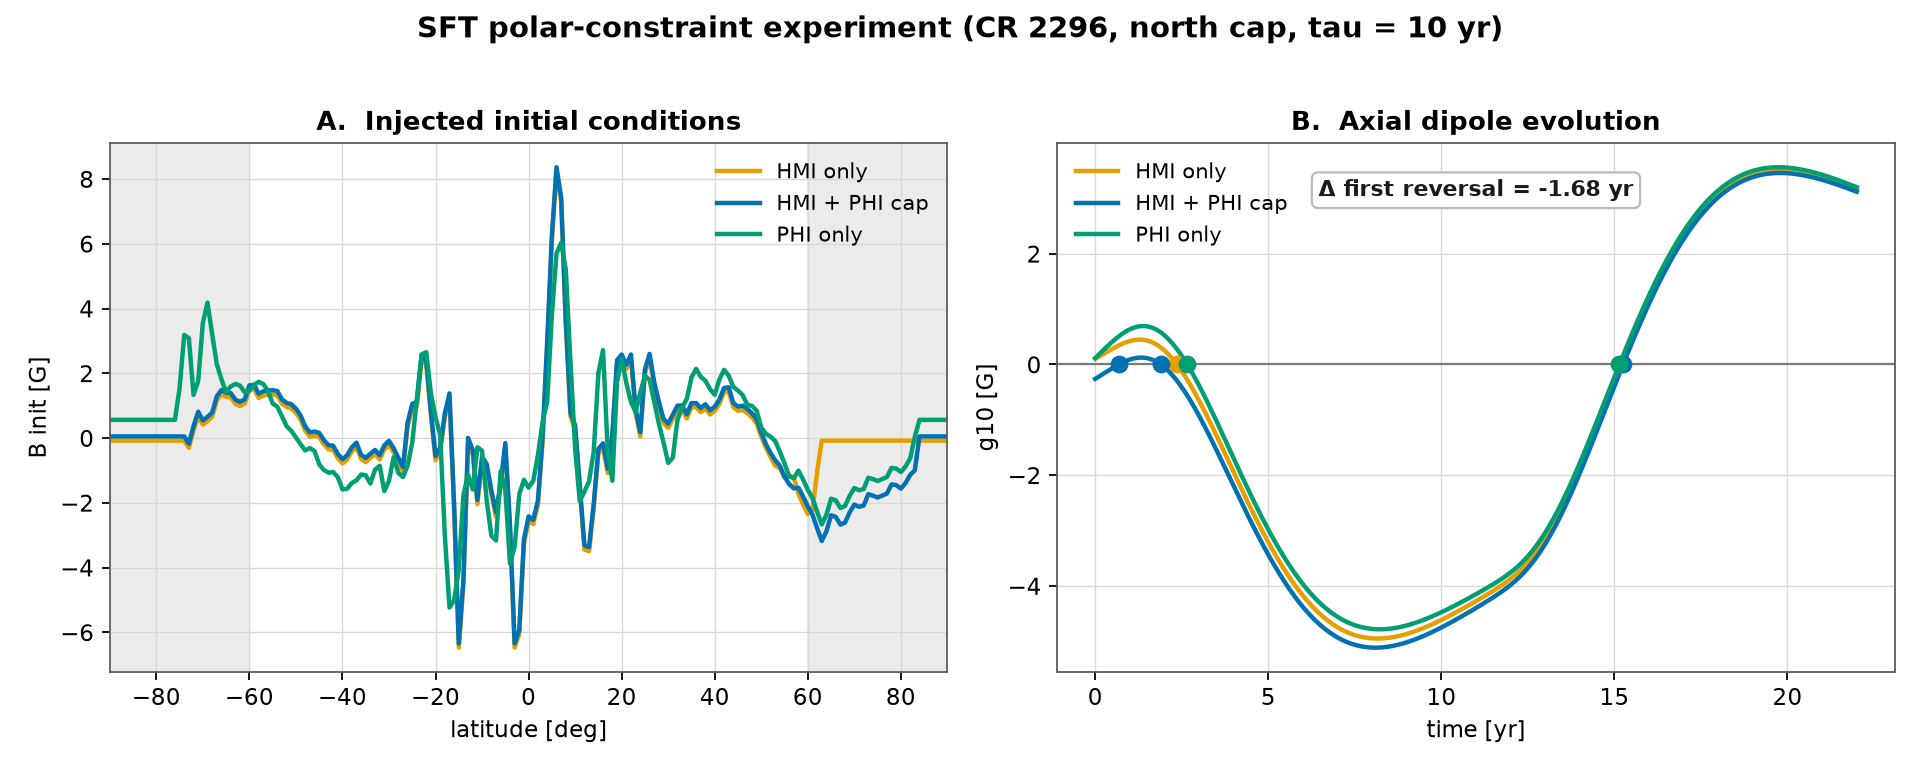
\includegraphics[width=0.85\textwidth]{figures/sft_polar_figure.png}
\caption{CR\,2296 north-cap polar-constraint experiment with $\tau=10$\,yr. Panel A shows the injected initial conditions; the HMI profile is nearly flat through the constrained cap, while the HMI+PHI splice carries the PHI cap field. Panel B shows the resulting $g_{10}(t)$. The first reversal moves from 2.36\,yr in the HMI-only run to 0.68\,yr in the HMI+PHI-cap run, a shift of $-1.68$\,yr.}
\label{fig:sft}
\end{figure*}

\subsection{Comparison with HMI polar-filled reference maps}
\label{sec:results-reference}

As a consistency check, the per-rotation products are compared with the standard HMI polar-filled synoptic series, \texttt{hmi.synoptic\_mr\_polfil\_720s} \citep{Sun2018}. The reference dipole remains near $-0.17$ to $-0.21$\,G during CR\,2294--2296, decreases to $-0.57$\,G by CR\,2298, and reaches $-0.52$\,G in CR\,2299 (Table~\ref{tab:reference}). This behaviour is consistent with the rebuilding of the negative cycle-25 axial dipole after polar reversal.

At the beginning of the window the true dipole is close to zero, and partial-coverage products are strongly affected by sampling. In project-fill mode, the PHI and HMI products are positive during CR\,2294--2297, while the reference is slightly negative. As the reference dipole strengthens, the products recover the correct sign. By CR\,2299, both PHI ($-0.21$\,G) and HMI ($-0.04$\,G) are negative, and in project-fill mode PHI is closer to the reference than HMI ($\Delta=+0.31$\,G versus $+0.48$\,G). This reference comparison should not be interpreted as an absolute truth test, since the reference itself contains a polar-fill model. It is used only as an external consistency check.

\begin{table}
\caption{Axial dipole moment compared with the HMI polar-filled reference chart in project-fill mode.}
\label{tab:reference}
\centering
\footnotesize
\begin{tabular}{lccccc}
\hline\hline
Rotation & $g_{10,{\rm ref}}$ & $g_{10,{\rm PHI}}$ & $\Delta_{\rm PHI}$ & $g_{10,{\rm HMI}}$ & $\Delta_{\rm HMI}$ \\
\hline
CR\,2294 & $-0.21$ & $+0.47$ & $+0.68$ & $+0.35$ & $+0.57$ \\
CR\,2295 & $-0.17$ & $+0.98$ & $+1.15$ & $+0.34$ & $+0.50$ \\
CR\,2296 & $-0.18$ & $+0.56$ & $+0.74$ & $+0.17$ & $+0.36$ \\
CR\,2297 & $-0.39$ & $+0.29$ & $+0.68$ & $+0.12$ & $+0.50$ \\
CR\,2298 & $-0.57$ & $+0.11$ & $+0.67$ & $-0.01$ & $+0.55$ \\
CR\,2299 & $-0.52$ & $-0.21$ & $+0.31$ & $-0.04$ & $+0.48$ \\
\hline
\end{tabular}
\tablefoot{All values are in G. $g_{10,{\rm ref}}$ is from \texttt{hmi.synoptic\_mr\_polfil\_720s}; $\Delta_X=g_{10,X}-g_{10,{\rm ref}}$. The merged product has valid rows only for CR\,2294--2295; for CR\,2296--2299 the Solar Orbiter--Earth separation exceeds the merge guard.}
\end{table}

%-------------------------------------------------------------------
\section{Discussion}
\label{sec:discussion}

The main result is not simply that PHI can be added to HMI\@. Rather, the 2025 campaign shows that the PHI polar advantage and the validity of a PHI--HMI merge are controlled by different aspects of the geometry. Polar coverage is controlled by the heliographic latitudes of the observers, whereas the merge is controlled by their Carrington-longitude separation. Solar Orbiter reaches its most favourable polar-viewing geometry when it is also far from Earth in longitude. At those epochs the two instruments are not observing the same part of the solar surface.

This leads to a simple operational distinction. When the separation is small, as in CR\,2294 and part of CR\,2295, the PHI and HMI maps can be compared directly and a merged product is well posed. However, the polar advantage is then limited. When PHI observes the north polar cap most favourably, in CR\,2296--2297, the spacecraft are separated by $80^{\circ}$--$180^{\circ}$ and a per-pixel merge is not meaningful. In this regime, PHI should be used as an independent polar boundary constraint rather than as a co-registered merge partner.

The SFT experiments show why this distinction matters. A PHI north-cap constraint changes the early evolution of the axial dipole and shifts the first reversal by more than a year, whereas a PHI south-cap constraint in a cap already observed by HMI has essentially no effect. The value of the polar view is therefore localised in the missing information: it matters where the Earth view is blind. The separation guard makes this statement rigorous by preventing a merged map from being constructed when the two input maps sample disjoint hemispheres.

%-------------------------------------------------------------------
\section{Uncertainties and limitations}
\label{sec:uncertainties}

\begin{itemize}
    \item \emph{Line-of-sight-to-radial approximation.} The correction $B_r\simeq B_{\rm los}/\mu^{\alpha}$ is least reliable in strong active-region fields and near the limb. A quiet-Sun restriction ($|B_r|\le50$\,G) reduces the cross-vantage project-mode difference. Vector-field products would remove this approximation.
    \item \emph{Calibration slope.} The sub-unity PHI-versus-HMI slope is largely explained by resolution-dependent cancellation of fine mixed-polarity structure. Smoothing HMI to the PHI scale brings the slope to unity and increases the correlation, but residual programme-dependent effects remain.
    \item \emph{Limb cut.} The magnitude of the polar-coverage advantage depends on $\mu_{\rm min}$. At $\mu_{\rm min}=0.4$, the CR\,2296 north-cap ratio is about $16\times$; at $\mu_{\rm min}=0.25$ it falls to about $2.6\times$. The sign of the advantage remains the same.
    \item \emph{Longitude coverage.} Individual rotations have incomplete longitude coverage, and this dominates the uncertainty on the absolute 2025 $g_{10}$ values. Coverage statistics and differential product comparisons are more robust.
    \item \emph{Polar filling.} The fill mode remains a major uncertainty on the absolute dipole. For this reason, the zero, project, and polar-extension estimates are reported separately where relevant.
    \item \emph{Polar-splice prescription.} The SFT polar-constraint experiments use a smooth latitudinal splice between the HMI profile and the PHI-observed cap. The sensitivity to the cap boundary and ramp width should be explored in future work.
    \item \emph{Axisymmetric SFT.} The SFT experiments use a one-dimensional model and a single initial-condition injection. Longitude-dependent and time-dependent assimilation of PHI are left for future work.
\end{itemize}

%-------------------------------------------------------------------
\section{Conclusions}
\label{sec:conclusions}

\begin{enumerate}
    \item The CR\,2264 low-inclination window validates the pipeline. PHI and HMI agree on their common support with map-space correlation $r\simeq0.89$ and $g_{10}$ agreement at the level of $\simeq0.05$\,G.
    \item During the 2025 high-$B_0$ campaign, PHI's reliable polar-cap coverage exceeds HMI's by up to a factor of 16. The advantage appears in the south cap when Solar Orbiter is at negative heliolatitudes and in the north cap when it reaches positive heliolatitudes.
    \item At the northern apex, PHI gives a negative north-polar contribution to $g_{10}$, while HMI gives a positive contribution from grazing-angle coverage. In project-fill mode, PHI is also closer than HMI to the HMI polar-filled reference by CR\,2299.
    \item The largest polar advantage occurs at the largest Solar Orbiter--Earth separations. At the decisive epochs, the merged product is therefore invalid. PHI is best used as a standalone polar constraint, not as a co-registered merge partner.
    \item Replacing the poorly observed HMI north cap with the PHI-derived cap shifts the first SFT-predicted reversal by $-1.68$\,yr in CR\,2296 and by $-1.26$\,yr in CR\,2297. Replacing the co-observed south cap changes the timing by only $-0.004$\,yr.
    \item The method, its main systematics, and the open-source tools are established end to end, from data preparation to polar-constrained SFT experiments.
\end{enumerate}

%-------------------------------------------------------------------
\begin{acknowledgements}
The author thanks the Solar Orbiter/PHI and SDO/HMI instrument teams for making the data used in this work publicly available.
\end{acknowledgements}

\paragraph{Data availability.}
The SO/PHI-FDT magnetograms are publicly available from the ESA Solar Orbiter Archive (SOAR, \url{soar.esac.esa.int}). The SDO/HMI magnetograms are publicly available from the Joint Science Operations Center (JSOC, \url{jsoc.stanford.edu}). The open-source analysis pipeline, baseline configuration, and scripts used to reproduce the results are available at \url{https://github.com/mtalafha90/SO-PHI-SDO-HMI}.

\bibliographystyle{aa}
\bibliography{references}

\end{document}
